\chapter[Referencial Teórico]{Referencial Teórico}

Neste capítulo será abordado como funciona os temas tratados neste trabalho, bem como introduzir conceitos importantes para a melhor compreensão do tema.

\section{A base da robótica}

O termo robô foi criado em 1921 pelo dramaturgo tcheco Karel Capek, em sua obra \textit{Rossum’s Universal Robots}, sendo o  termo uma variação da palavra \textit{robota} (trabalho forçado) (Mataric, 2007, p.18). Na obra os robôs eram máquinas humanoides que realizavam todo tipo de trabalho, porém o conceito do que é um robô tem sofrido variações ao longo do tempo. 

\subsection{Definição de robótica}

Mataric (2007) e Abreu (2001) consideram máquinas movidas por engrenagens e vapor séculos antes como ancestrais dos robôs atuais por suas articulações e movimentos por vezes independentes de interação humana. Hoje ainda não há um consenso do que exatamente pode se enquadrar como robô. Segundo a RIA (Associação das Indústrias de Robótica), um robô industrial é um "manipulador reprogramável, multifuncional, projetado para mover material, ferramentas ou dispositivos especializados através de movimentos programáveis variados para desenvolver uma variedade de tarefas". Abreu (2001) apresenta mais definições de robôs industriais. 

Mataric (2007) apresenta uma definição mais genérica, que abrange não só robôs industriais, mas todos os grupos, segundo ele "um robô é um sistema autônomo que existe no mundo físico, que reconhece o ambiente a volta e poder agir sobre ele para alcançar suas metas".

Segundo Secchi (2008) existem três tipos de robôs: industriais, médicos e móveis, apesar das demais bibliografias fazerem referência apenas aos robôs industriais e móveis.

\subsection{Robôs industriais e móveis}

A robótica industrial foi a que impulsionou a pesquisa e desenvolvimento na área de robótica. Ela criou um mercado bilionário ao redor do mundo desenvolvendo soluções automatizadas para a indústria. Esses robôs em grande parte eram braços robóticos que realizavam trabalhos perigosos e/ou repetitivos com grande precisão e velocidade. 

Também chamados de manipuladores, os braços robóticos eram fixos em uma posição, formados por uma estrutura articulada que move a ponta para o local desejado para trabalhar. Os graus de liberdade das articulações e o comprimento dos braços que os ligavam definem a área de atuação do robô, que são classificadas pelo formato alcançado por ele (cartesiano, cilíndrico, esférico...). Normalmente as máquinas possuem seis graus de liberdade (um para cada articulação), três para posicionar a ponta de trabalho no local certo e mais três para movê-la ao executar o serviço (Abreu, 2002).

\begin{figure}[h]
	\centering
	\label{fig01}
		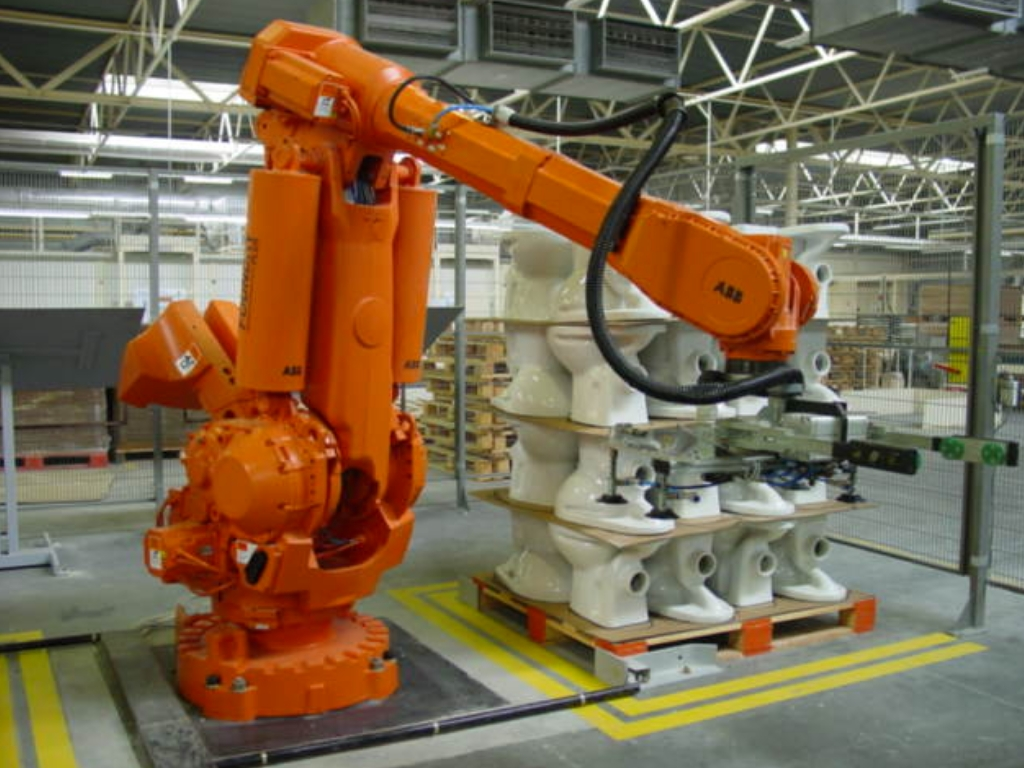
\includegraphics[keepaspectratio=true,scale=0.6]{figuras/1bracorobotico.jpg}
	\caption{braço robótico usado na robótica industrial}
\end{figure}

Já a robótica móvel, por sua vez, trata de máquinas capazes de se movimentar independentemente. Com maior liberdade de movimentação, este grupo de máquinas possui uma maior gama de trabalhos. Um robô móvel pode ser terrestre, aquático, voador ou até espacial (VIEIRA, 2005, p.), sendo movidos por rodas, esteiras, patas, hélices, etc. Com essa ampla área de atuação e o dom da mobilidade, podemos encontrá-los aplicados nas mais diversas áreas. Pereira (2003) lista cinco grandes áreas aonde eles são mais utilizados: indústria, serviços, pesquisa, campo e entretenimento.

\subsection{Estruturas físicas de robôs com rodas}

Existe um grande campo de pesquisa para cada forma de deslocamento do robô. No caso dos robôs com rodas, o tipo de roda e a estrutura do chassi são consideradas para a mobilidade que a máquina terá. Siegwart (2004) afirma que é possível dar estabilidade ao robô com duas ou três rodas e ao usar quatro ou mais é necessário um sistema de suspensão para permitir que todas as rodas toquem o chão quando o robô estiver em terreno acidentado.

Secchi (2008) lista quatro tipos de roda mais usados: rodas fixas para tração, roda orientável centralizada para direção e tração, roda castor (ou roda louca) para estabilidade e a suéca para mobilidade. Já Rolland (2004) lista outras quatro: a roda padrão (semelhante a orientável centralizada), a castor, a suéca e a esférica, que assim como a suéca permite maior mobilidade.

\begin{figure}[h]
	\centering
	\label{fig02}
		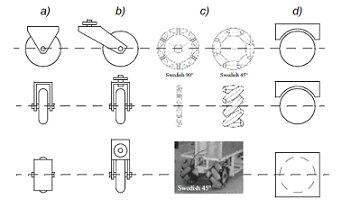
\includegraphics[keepaspectratio=true,scale=1]{figuras/1rodas.png}
	\caption{a) roda padrão, b) roda castor, c) roda suéca d) roda esférica}
\end{figure}

A definição das rodas determina a quantidade de liberdade de movimento da estrutura. Para fazer um robô omnidirecional (que se movimenta para todos os lados sem reorientação) por exemplo costuma-se usar rodas suécas ou esféricas, porém também é possível montar com rodas orientáveis centralizadas (Secchi, 2008). Ele se destaca por sua capacidade de se mover em qualquer sentido (frente, trás, lados e girar em torno do próprio eixo) usando um motor para cada roda. Robôs do tipo \textit{Synchro Drive} também podem se mover para qualquer direção, porém ao contrário do omnidirecional que tem um motor para cada roda, esse usa três rodas ligadas ao mesmo motor, girando-os com a mesma velocidade e mesma direção (Borenstein, 1996). Esses tipos de robô são chamado holonômicos.

Secchi e Borenstein também apresentam máquinas do modelo triciclo, que possuem uma roda orientável centralizada afrente e duas convencionais presas ao mesmo eixo atrás, como as rodas de trás de um carro. A roda da frente tem função de direcionar e de tração, enquanto as duas traseiras apenas acompanham o movimento. Outro modelo semelhante é o modelo de quadriciclo, que funciona igual a um carro, com duas rodas de tração-direção na frente ligadas ao mesmo motor e atrás duas rodas de tração também presas ao mesmo eixo. 

Ambos os modelos acima sofrem erros de odometria (estimação da posição do robô) e apresentam problemas de derrapagem em curvas. Essa derrapagem ocorre pelo fato da roda interna à curva fazer um arco menor que a roda externa, obrigando essa a derrapar e desgastar o pneu. Esse problema pode ser consertado com um modelo chamado \textit{Ackerman Steering}. Segundo Borenstein (1996), Secchi (2008) e Bagnall (2011) o sistema \textit{Ackerman} inclina mais uma roda que a outra para compensar a diferença de espaço percorrido, fazendo com que o eixo de cada roda sempre esteja apontando para o centro da curva, conforme a Fig.3 mostra.

\begin{figure}[h]
	\centering
	\label{fig03}
		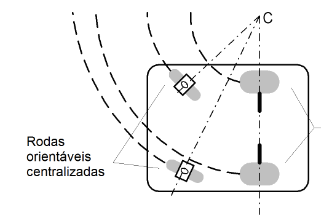
\includegraphics[keepaspectratio=true,scale=1]{figuras/2ackerman.png}
	\caption{Ackerman Steering}
\end{figure}

Robôs do tipo \textit{differential steering} possuem três rodas: duas fixas para guiar o robô e uma roda castor atrás para dar estabilidade. O grande diferencial desse modelo é que cada roda de direção possui um motor separado. As duas rodas estão alinhadas no mesmo eixo, porém diferente de um carro onde ambas estão ligadas ao mesmo motor, cada uma é independente com seu próprio motor. Isso o permite girar em torno do próprio eixo e não depender de manobras em arco como o modelo de carro (Bagnall, 2011) (Secchi, 2008) (Mataric, 2007).

\section{Robótica a nível de software}

A nível de software a robótica móvel apresenta diversos desafios a serem superados. Dotar uma máquina com a capacidade de locomover-se sozinha esconde diversas dificuldades, que advém do fato de que a navegação deve integrar sensoriamento, atuação, planejamento, arquitetura, hardware, eficiência e computação (Souza, 2008). A navegação do robô por um terreno envolve mapeamento da região, controle dos motores, sensoriamento, auto-localização e definição de trajetória. Uma visão geral sobre cada uma é dada a seguir para ajudar a compreender o trabalho de navegação como um todo e a importância de cada um.

\subsection{Dificuldades da robótica móvel}

A primeira dificuldade da navegação de um robô é a correta locomoção do robô. Podemos determinar o movimento do robô com cálculos pesados para o controle mecânico dos motores, considerando os tipos de rodas e distribuição do peso. O controle matemático do robô é dividido em controle cinemático (não considera efeitos dinâmicos provocados pelo movimento do robô, como atrito e derrapagem) e dinâmico (considera efeitos provocados pelo movimento, como atrito e derrapagem). A determinação do movimento e orientação da máquina é feita por uma série de equações e por operações lineares e vetoriais, considerando os planos cartesianos e a direção para onde aponta o robô (Siegwart, 2004).

Outro desafio é definir a real posição da máquina. A locomoção nem sempre ocorre como esperado. Derrapagem, atoleiros e forças externas que empurram o robô geram uma mudança da sua real posição com a esperada inicialmente. A odometria procura obter incrementalmente informações do movimento do robô, lendo o número de rotações que cada roda deu para determinar a localização final. Porém essa solução possui alto índice de erros cumulativos que o tornam inadequado para longas distâncias (Pereira, 2003). Outras soluções são a de \textit{beacons} (faróis), que se comunicam com o robô dando sua coordenada dentro daquela região mapeada. O sistema de \textit{beacon} mais abrangente é o de GPS, porém faróis locais também são comuns para localização dentro de áreas pré-determinadas. Marcas no chão para auto localização pelo robô também são muito usados em ambientes fechados. Outra solução é através de processamento de imagens, onde o robô conhece alguns objetos ou locais únicos e suas posições no mapa e ao passar por eles sabe onde está. Borenstein (1996) explica cada um dos algoritmos de localização mais aprofundado.

O mapeamento consiste na modelagem do ambiente que contém o robô através do uso de mapas obtidos pelo sistema sensorial ou previamente armazenados (Souza, 2008). Considerando o sensoriamento, a forma de escanear a região depende muito dos tipos de sensores usados e seu alcance. Uma representação do mundo real dentro da máquina ajuda muito nas tomadas de decisão apesar de ocupar muita memória.

A definição do caminho a ser percorrido também gera um desafio. Apesar de ser algo complexo, não necessariamente é mais crítico ou mais difícil que os anteriores. Porém, por ser o tema deste trabalho, será abordado mais profundamente que os demais no tópico a seguir.

\subsection{Paradigmas de definição de trajetória}

Há duas estratégias mais abordadas para a definição de trajetórias: uma em que o robô não conhece nada ao seu redor (algoritmos locais) e uma em que o robô conhece previamente todo o ambiente (algoritmos globais).

Berenguel (2008) explica que os algoritmos locais o robô procura seguir em linha reta até um ponto desejado e ao encontrar um obstáculo ele contorna o objeto até que não detecte mais nada entre ele e o ponto final. Neste tipo de algoritmo a comunicação com os sensores de presença se fazem essencial. Um problema deste paradigma é encontrar um mínimo local, aonde o robô entra mas não consiga sair (Souza, 2008, p.22). Secchi (2008) explica o funcionamento de alguns métodos locais. 

Dentre os algorítmos locais, um que vale ser comentado é o algorítmo potencial, comentado por Secchi (2008), Souza (2008), Berenguel (2008), Choset (2005), Siegwart (2004) e Thomsen (2010). Este algorítmo funciona sem uma rota pré-definida e, ao invés disso, usa uma ideia de atração e repulsão para se locomover. O objetivo tem um efeito atrativo, puxando o robô para sua direção enquanto os obstáculos tem efeito repulsivo, distanciando o robô de si. Como o ponto final é conhecido desde o início ele tem seu efeito atrativo funcionando a todo instante enquanto o efeito repulsivo dos obstáculos só ocorre quando o obstáculo está ao alcance dos sensores.

Nos algoritmos globais o robô possui um mapa interno com os obstáculos presentes e define rotas entre eles para chegar ao outro ponto (Berenguel, 2008) (Souza, 2008). Esta estratégia não precisa conhecer os sensores, porém envolve maior modelagem do ambiente a sua volta e dos objetos que tem nela. Uma outra camada que, essa sim, conhece os sensores, pode realizar o sensoriamento e entregar o mapa pronto ao módulo. Os algoritmos globais serão melhor explicados mais a frente.

Os dois podem ser usados juntos para obter melhores resultados, usando o global para definir o caminho completo, traçando longas distâncias, e o local para a movimentação a curta distância, verificando mudanças no ambiente próximo com os sensores para correções naquela parte (Souza, 2008). Outros autores como Secchi (2008) também apresentam a mesma ideia.

Mataric (2007), por sua vez, apresenta quatro tipos de algoritmos para planejamento de trajetória: os deliberativos, reativos, híbridos e baseado em comportamento. Berenguel (2008) descreve navegação deliberativa como a mesma coisa que os algoritmos globais e a reativa como o mesmo que os algoritmos locais.

Os deliberativos conhecem o mapa todo previamente e fazem toda a análise antes de agir. Essa análise prévia é descrita como o grande problema desse paradigma, pois o robô precisa ficar muito tempo parado para tomar a decisão. "Se o problema exige uma grande dose de planejamento antecipado e não envolve nenhuma pressão de tempo, e, ao mesmo tempo que apresenta um ambiente estático e baixa incerteza na execução, então esse paradigma atende bem ao caso" (Mataric, 2007, p.175). 

Os reativos possuem a mesma descrição que os algoritmos locais definidos por Berrenguel, Souza e os demais autores. "Ele é baseado em uma estreita ligação entre os sensores e atuadores do robô. Sistemas puramente reativos não usa quaisquer representações internas do ambiente. Eles operam em uma escala de tempo curto e reagem à informações sensoriais atuais." (Mataric, 2007, p.179). Isso os dá agilidade de processamento, porém não garante confiabilidade.

A navegação híbrida é uma mistura dos dois. A ideia básica por trás dele é obter o melhor dos dois mundos: a velocidade de controle reativo e os cérebros de controle deliberativo. Isso é alcançado através de três camadas, um planejador deliberativo, um reativo que comunica com os atuadores e uma intermediária ligando as duas. Essa solução usa os algoritmos deliberativos para longas distâncias (definindo o percurso de forma macro até o ponto final) e os reativos para distâncias curtas, entre cada ponto do percurso. Como já dito acima, Souza dá uma descrição parecida de navegação híbrida, apesar de não usar essa nomenclatura. O problema desta solução é a dificuldade de implementá-la.

Por fim, os algoritmos baseados em comportamentos são diferentes dos dois anteriores, dividindo suas funcionalidades em módulos que executam ações específicas que realizam um comportamento desejado, como andar para frente até encontrar um obstáculo ou seguir uma parede. O objetivo deste paradigma é montar ações que executam esse comportamento e fazer esses módulos criados se comunicarem. Esse paradigma, assim como o reativo, também precisa conhecer os sensores, que são a principal entrada dos módulos.

Há outros métodos de definição de trajetória. Berenguel (2008) comenta rapidamente sobre a existência de métodos probabilísticos e Strandberg (2004) descreve o método probabilístico baseado em \textit{roadmaps}.

\subsection{Visão geral sobre navegação}

Vieira (2005) define uma arquitetura de navegação de robôs móveis, onde cada camada é uma área de pesquisa e juntas realizam a navegação do robô. A primeira é a percepção do ambiente pelo robô, através de sensores. Após tratar esses dados e saber o que o cerca, é executada a camada de decisão, onde a máquina avalia a informação e decide que ações tomar. Essa camada é o cérebro do robô e pode possuir algoritmos de inteligência artificial nela.

\begin{figure}[h]
	\centering
	\label{fig04}
		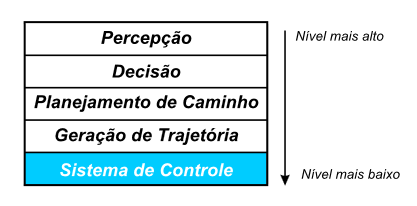
\includegraphics[keepaspectratio=true,scale=1]{figuras/arqRoboMoveis0.png}
	\caption{camadas de execução na navegação do robô}
\end{figure}

A camada de planejamento de caminho é a que define por onde o robô irá passar para chegar a posição desejada. É nesta camada que será feito o trabalho. Com o ambiente já reconhecido pelas camadas acima e o controle do hardware pelas camadas abaixo, o sistema proposto (assim como a camada descrita por Vieira) define um percurso por onde a máquina não chocará com os obstáculos detectados considerando o tamanho do robô. Existe uma série de algoritmos que fazem a  escolha do melhor caminho livre de obstáculos e no \textit{framework} será implementado alguns deles para uso comum a todos os desenvolvedores interessados.

A camada abaixo é a de definição de trajetória. Ela pega o caminho definido pela camada de cima e define que ações devem ser feitas sobre o hardware para percorrer aquele percurso. Essa camada deve conhecer a estrutura do robô e suas limitações físicas de movimento. Ela define a velocidade e direção em que o robô irá andar, repassando aos motores os sinais necessários a cada instante do percurso. 

A última camada é a que atua diretamente no hardware, garantindo que os atuadores estão recebendo o sinal certo para girar conforme desejado.

Bagnall (2011) também apresenta uma arquitetura de navegação muito interessante baseada na navegação de um navio. Ele define que um sistema de navegação deve possuir: um veículo (hardware), piloto (controlador dos motores), navegador (gerador do caminho), provedor de posição (algoritmos de auto-localização), mapas, planejador de trajetória (algoritmos de definição de trajetória)  e planejador da missão.

O veículo é o hardware do robô, que precisa ser manipulado para sair de um ponto a outro. Assim como cada navio é diferente, cada hardware também é, tanto por sua estrutura quanto pelos motores e sensores utilizados.

O piloto é quem controla o veículo diretamente. No caso da robótica será a camada mais baixa, que controla os motores e realiza o controle cinemático.

O navegador já não conhece detalhes do navio (hardware), apenas atua como homem-do-meio entre o piloto e os líderes do navio. Ele que diz ao piloto que devem se mover do ponto X ao ponto Y, transformando o sistema de coordenadas conhecido em comandos que o piloto (máquina) saiba interpretar. Ele não funciona sem um sistema de coordenadas definido e sem saber sua posição atual. Ele seria a penúltima camada da arquitetura apresentada por Vieira.

O provedor de posição é quem opera a bússola do navio, especialista em responder aonde estão. No robô são os algoritmos de localização como odometria e uso de \textit{beacons} e faz parte do sensoriamento (camada de percepção).

O mapa informa os obstáculos e o sistema de coordenadas para a tripulação, estando lá para ser analisado sempre que preciso.

O planejador de trajetória é quem trabalha acima do navegador. O navegador sabe como ir de um ponto a outro, gerando uma trajetória apenas entre dois pontos com movimentos mecânicos. Para realizar uma viagem grande, evitando obstáculos do mapa é preciso um planejador de trajetória. Ele estuda o mapa e desenha um percurso seguro com os pontos que devem ser atravessados.

Por fim o planejador de missão é o capitão do navio. Na robótica pode ser o cérebro do robô caso haja uma inteligência artificial ou o próprio programador, que define par aonde se deve ir e o porquê.

Mataric (2007) define uma arquitetura para cada paradigma de definição de trajetória que apresenta. Para algoritmos globais (deliberativos) ele apresenta a arquitetura SPA (\textit{sensor-plan-act}), que funciona em três camadas. A camada "\textit{sensor}" cuida do mapeamento e sensoriamento (como a primeira camada de Vieira), a camada "\textit{plan}" define a trajetória e pesa os critérios de decisão (como a segunda e terceira camada) e a camada "\textit{act}" que se comunica com os motores e realiza o movimento (como as últimas camadas).

\begin{figure}[h]
	\centering
	\label{fig05}
		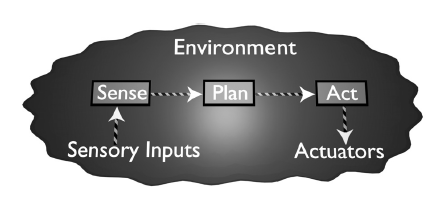
\includegraphics[keepaspectratio=true,scale=0.6]{figuras/6arquiteturaSPA.png}
	\caption{arquitetura SPA}
\end{figure}

\section{Mapeamento e modelagem dos obstáculos}

Um mapa é uma representação do mundo real dentro da memória do robô. Isso permite um conhecimento prévio da região e agiliza a tomada de decisão, além de permitir um pensamento mais a longo prazo (Mataric, 2007). 

Choset (2005) descreve três formas de construir um mapa: topologia, geometria e por malhas. Um mapa topológico é baseado em grafo, onde cada nó representa um local distinguível e as arestas são o caminho entre um local e outro. Qualquer ponto que possa ser diferenciável (uma sala, uma encruzilhada, uma marca no chão...) pode ser um nó. Mataric (2007) descreve os mapas topológicos como um mapa baseado em "\textit{landmarks}" (marcas). Por ser baseado nas características físicas do ambiente, as arestas ligando estes pontos não necessariamente são uma linha reta ou um corredor a ser seguido, mas uma série de movimentos que o leva até aquele ponto (segue reto, vira na primeira a direita e à esquerda na junção em "T").

O modelo geométrico usa formas geométricas para representar o ambiente (Choset, 2005). Ele detecta o ambiente e os obstáculos com maior detalhamento e define um objeto com o formato mais próximo do real. 

O modelo de malha de ocupação (\textit{occupancy grid}) divide o espaço em uma matriz, onde cada célula representa um pequeno pedaço do ambiente e seu valor a propabilidade daquela célula está ocupada. Borenstein (1996) lista as vantagens e desvantagens da malha de ocupação, essa abordagem permite maior densidade de dados, requer menos processamento ao longo da definição de trajetória e é mais fácil de criar, porém possui áreas de incerteza, tem dificuldades com obstáculos dinâmicos e exige um processo de estimativa complexo.

O problema do mapeamento é o gasto de memória, que nem sempre é algo muito disponível em um robô. Uma forma de diminuir isso é mapear apenas aquilo que os sensores são capazes de detectar e desconsiderar detalhes que não estejam ligados com a posição. Relevo só é considerado quando a locomoção do robô for impedida por ele. Outra forma de economizar espaço, comentada por Siegwart (2004) e Berenguel (2008) é descartar áreas côncavas nos obstáculos, ligando os vértices mais próximos que formem uma região convexa e considerando toda a área livre entre os pontos como região de risco e, portanto, intransponível.

Porém, mesmo abstraindo o máximo de informações, o espaço ocupado na memória ainda será proporcional a quantidade de obstáculos na região. Assim, quanto mais denso de objetos for o mapa mais memória será ocupada e mais processamento será exigido (Siegwart, 2004).

Há duas abordagens para a busca pelo menor caminho nos mapas, os \textit{roadmaps} e a decomposição celular.

Um \textit{roadmap} é um mapa com um conjunto de posições específicas livres (nós). O \textit{roadmap} que liga duas posições através de um caminho livre. Choset (2005) define um \textit{roadmap} como uma classe de mapa topológico e o compara como um mapa de uma auto-estrada, que liga locais específicos por caminhos que se possam trafegar formando um grafo.

A decomposição celular porém funciona dividindo o mapa em regiões livres, aonde qualquer lugar dentro daquela região é navegável. As regiões vizinhas são deslocáveis de uma para outra, podendo passar pela borda entre eles sem problemas. Assim, os algoritmos que usam essa abordagem ligam as regiões vizinhas como nós adjacentes em um grafo, dizendo que aquelas duas regiões são trafegáveis entre si. As regiões podem ter todas o mesmo tamanho ou variar drasticamente, mas devem sempre caber o robô em seu interior.

A decomposição celular é dividida em dois sub-gupos: a exata, aonde cada região tem exatamente o formato da área livre, sem deixar nenhuma parte do mapa fora de uma das regiões; e a aproximada, aonde cada região tem um formato pré-determinado (embora o tamanho possa ser variável) e pode desconsiderar pequenas partes do mapa, causando possíveis perdas de trajetos (Souza, 2008).

\section{Algorítmos globais de definição de trajetória}

Como comentado anteriormente, o foco do trabalho será na definição de trajetória usando algoritmos globais. Esse grupo de algoritmos já conhecem o ambiente, tendo um mapa da região e dos obstáculos presentes. A partir deste mapeamento é definido uma trajetória para o robô percorrer sem colidir com nenhum dos obstáculos. Os obstáculos serão considerados estáticos para este trabalho.

Para fazer essa análise, os algoritmos transformam o mapa em um grafo e depois rodam um algoritmo de melhor caminho nele (como por exemplo Djikstra ou A*) para definir a trajetória. Cada algoritmo gera um grafo diferente e, portanto, uma trajetória diferente. Porém após definido o grafo todos funcionam de forma semelhante, rodando o algoritmo de Djikstra ou semelhante para solucioná-lo e criar o percurso (Berenguel, 2008). O diagrama de sequência abaixo ilustra esse funcionamento, onde a classe PathPlaning representa a classe do sistema projetado que abstrai o funcionamento.

\begin{figure}[h]
	\centering
	\label{fig06}
		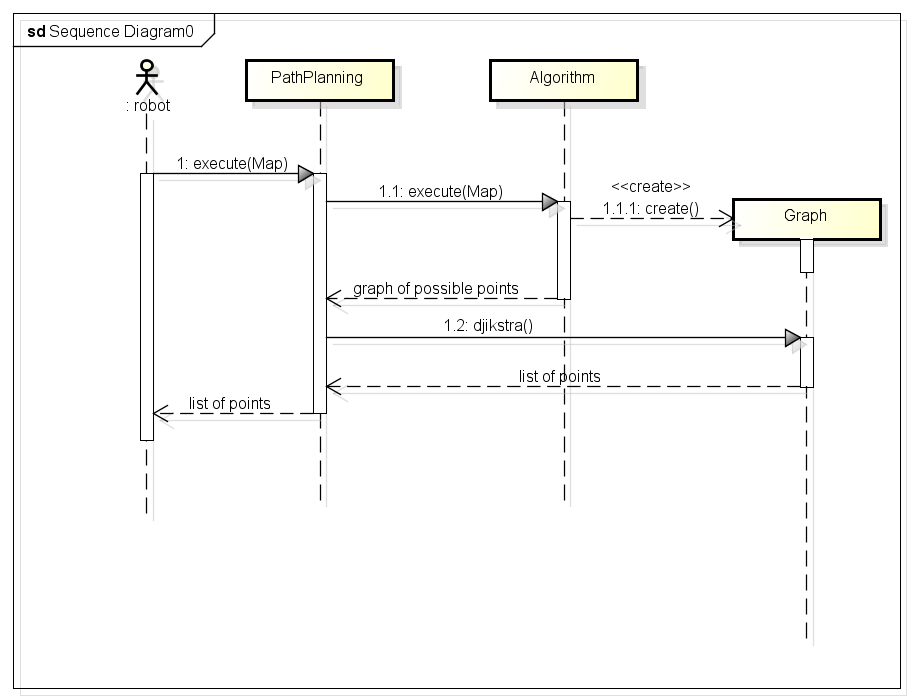
\includegraphics[keepaspectratio=true,scale=0.6]{figuras/5diagramaSequencia.png}
	\caption{diagrama de sequência da criação do caminho}
\end{figure}

Assim, a camada de planejamento de trajetória recebe das camadas acima um mapa com obstáculos, deve ter acesso a estrutura do robô (como seu tamanho) e passa para as camadas abaixo uma lista de pontos que o robô deverá seguir. Será esta lista de pontos (nós do grafo definidos pelo algoritmo de melhor caminho) que formarão a trajetória, cabendo a camada abaixo o controle dos motores para ir de um ponto ao outro.

Os algoritmos globais estão divididos em dois grupos, cada um utilizando uma abordagem para trabalhar com o mapa: os \textit{roadmaps} (Grafo de Visibilidade, Voronoi) aonde o grafo representa um conjunto de caminhos livres ligando posições específicas do mapa, e a decomposição celular (Quad Tree e Wavefront) aonde o espaço é dividido em regiões geométricas menores livres e ocupadas e liga essas regiões se for possível se deslocar entre elas (Souza, 2008).

\subsection{Grafos de Visibilidade}

Grafo de Visibilidade é baseado no conceito de pontos visíveis, que são pontos (inicial, final e vértices dos obstáculos) que podem ser ligadospor uma linha reta sem passar por nenhum obstáculo (Berenguel, 2008). Em outras palavras, se alguém estiver parado em um ponto, ele estará ligado a todos os pontos que conseguir enxergar dali. Souza (2008) diz que a complexidade de um Grafo de Visibilidade depende da complexidade da geometria de seus obstáculos.

Este método permite alcançar sempre o menor caminho, porém ele passa sempre o mais perto possível dos obstáculos. Como o robô é considerado como apenas um ponto (seu centro) ele se chocaria aos vértices dos obstáculos. Para evitar isso Souza (2008), Siegwart (2004) e Thomsen (2010) dizem que os obstáculos devam ser expandidos, sendo considerados maior do que realmente são. Essa margem de erro deve ser maior que metade da largura do robô para que não haja contato.

Segundo Thomsen (2010) e Choset (2005) a complexidade deste algorítmo é O(n3), sendo O(n) para saber se dois vértices são visíveis ou não e O(n2) para percorrer todos os vértices e executar este algoritmo em todos os possíveis vizinhos. Thomsen (2010) diz que ele pode ser diminuído para o(n2 log n). Medeiros (2011) sugere um método para descartar nós e arestas sem prejudicar o resultado final e Choset (2005) apresenta um método para descarte de arestas dentro de uma região. Siegwart (2004) comenta que por gerar demasiados vértices e arestas, este algorítmo funciona melhor em ambientes esparsos, gerando menor gasto de processamento.

\begin{figure}[h]
	\centering
	\label{fig07}
		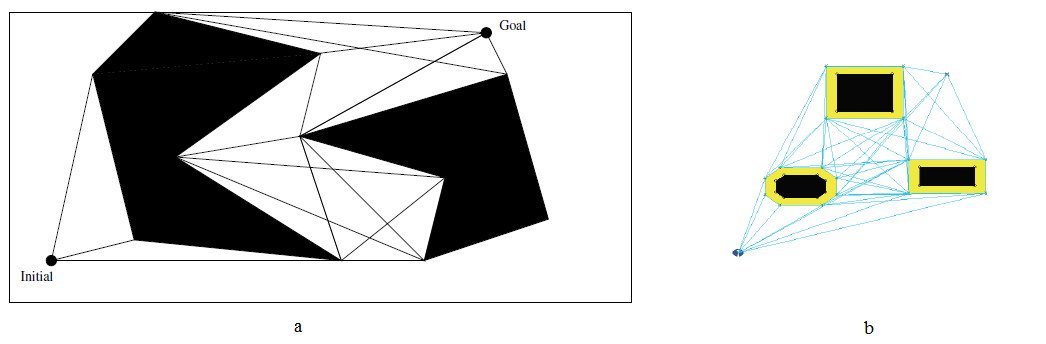
\includegraphics[keepaspectratio=true,scale=0.6]{figuras/7visibilityGraph.png}
	\caption{grafos de visibilidade a) tradicional b) com expansão dos obstáculos }
\end{figure}

\subsection{Voronoi}

O Diagrama de Voronoi é utilizado em diversos contextos diferentes. É possível encontrar aplicações dele na geofísica, química, na meteorologia, biologia, entre outros (http://www.Voronoi.com).

O diagrama consiste em dividir a região em áreas poligonais menores chamadas células, aonde cada ponto de uma célula esteja mais pŕoximo do seu centro do que do centro de outra célula. Cada célula é definida a partir deste ponto central, que deve está igualmente distante dos obstáculos e dos limites do mapa (Berenguel, 2008). Devido a essa característica ele gera um caminho maior entre o ponto inicial e final, porém garante que passará longe de qualquer obstáculo, dando prioridade a segurança do que ao percurso.

Siegwart (2004) e Choset (2005) comentam que essa abordagem possui um risco agregado. Por buscar sempre o caminho mais distante dos obstáculos, caso o robô não possua sensores de longo alcance ele não poderá confirmar sua posição exata. Sem obstáculos e objetos para captar o robô não terá o que usar para estimar sua posição atual e terá de percorrer o percurso sem ter certeza de onde exatamente está ou se permanece no percurso correto.

Para montar as células, o algoritmo primeiramente precisa receber um conjunto de pontos, que são os vértices dos obstáculos. Com estes pontos, o algoritmo executa um algoritmo de triangulação para determinar o ponto central do triângulo e a partir deles o centro de cada célula. A triangulação de Delaunay é a opção mais comum ao Diagrama de Voronoi (Souza, 2008). Após realizar a triangulação, são excluídos as interceções com obstáculos e triângulos formados dentro dos mesmos. Por fim são adicionados os pontos inicial e final e ligados aos centros das células próximas. Ao rodar um algorítmo de menor percurso (Djikstra ou A*) ele passará por estes pontos, sempre pelo meio das células até o objetivo.

\begin{figure}[h]
	\centering
	\label{fig08}
		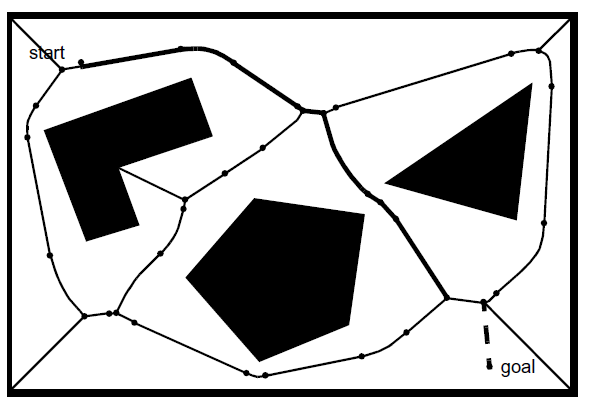
\includegraphics[keepaspectratio=true,scale=0.6]{figuras/8voronoi.png}
	\caption{Diagrama de Voronoi}
\end{figure}

\subsection{Quadtree}

A decomposição aproximada, também chamada de Quadtree, divide o mapa em regiões e executa um método recursivo para continuar dividindo cada região em áreas cada vez menores (Thomsen, 2010). Essa divisão recursiva pode parar de duas formas: ou quando chegar em um tamanho mínimo ou quando toda sua região estiver livre ou ocupada. Ainda segundo Thomsen (2010) esse método recebe este nome porque uma região é dividida em quatro células menores de mesma forma cada vez que se decompõe.

Assim, O método do Quadtree divide o mapa em áreas de formato pré-determinado, porém com tamanhos diferentes de acordo com o espaçamento entre os obstáculos. Isso pode gerar a perda de caminhos estreitos por serem colocadas na mesma área que uma parte do obstáculo. Isso pode ser resolvido diminuindo a área mínima de cada região, porém acarretará no aumento de memória gasta e tempo de processamento da solução do trajeto. Siegwart (2004) exemplifica este caso na figura abaixo.

\begin{figure}[h]
	\centering
	\label{fig09}
		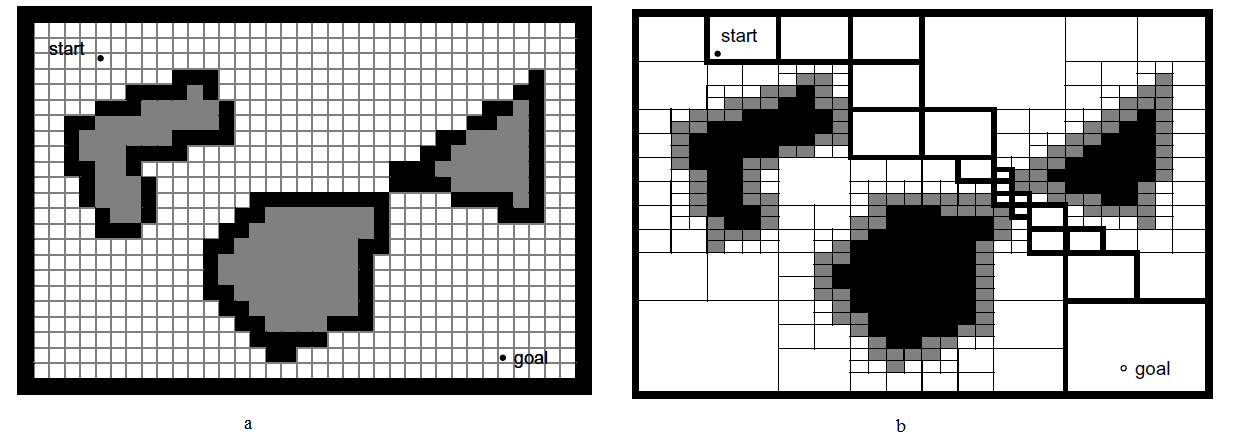
\includegraphics[keepaspectratio=true,scale=0.5]{figuras/9quadtree.png}
	\caption{ a) decomposição celular usando regiões de tamanho fixo b) Quadtree encontrando um caminho estreito entre dois obstáculos}
\end{figure}

Por fim, cada área será um vértice do grafo retornado e estará ligado a cada área adjacente livre.  Os vértices ocupados por obsáculos são retirados, permanecendo apenas os trajetos livres de uma área adjacente a outra.

\subsection{Wavefront}

O algoritmos Wavefront divide o mapa em pequenas células do mesmo tamanho e igualmente distribuídas, formando uma matriz de posições. Esse algorítmo funciona perfeitamente com mapas do tipo malha de ocupação, pois já está dividido em \textit{grids}. Cada célula possuirá um valor que representará o quão perto está da posição final.

O algorítmo começa na posição final e o dar uma valor inicial qualquer. Todas as casas em volta dele recebem o mesmo valor mais 1 as casas ao redor destes o valor delas mais 1. Assim, cada célula terá o valor inicial mais o número de passos para chegar até ele. Quando uma célula encontra um vizinho com um valor já estipulado ela troca seu valor apenas se o valor atual do seu vizinho for maior que o dela mesma mais um.

Este método permite chegar ao objetivo a partir de qualquer célula. Células com obstáculos são desconsiderados pelos vizinhos. 

Ao finalizar um grafo é feito ligando o ponto inicial à todas as células vizinhas com menor valor. Essas células por sua vez são ligadas às vizinhas com menor valor e assim por diante até todas as células passarem por essa função. Isso fará com que nem todas as células entrem no grafo, sendo inserido nele apenas os caminhos por onde o valor diminui. A imagem abaixo exemplifica a montagem do grafo.

\begin{figure}[h]
	\centering
	\label{fig10}
		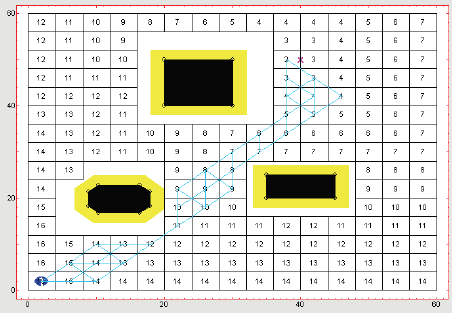
\includegraphics[keepaspectratio=true,scale=0.5]{figuras/10wavefront.png}
	\caption{algorítmo Wavefront, com grafo em azul}
\end{figure}

\section{Frameworks e padrões de projeto}

Escrever um código reutiizável e extensível não é fácil. Para garantir que o mesmo código possa ser replicado em diferentes contextos com nenhuma ou mínimo de alteração é preciso de uma arquitetura bem projetada e uma correta modularização das tarefas do sistema. Uma vez que é conhecido o escopo a ser atacado, um planejamento da melhor forma de estruturá-lo é necessário para garantir que todas as funcionalidades sejam separadas e suas comunicações o menos acopladas possível. Isso leva ao estudo de padrões arquiteturais, encapsulamento e padrões de projeto, que nos ajudam a realizar essa tarefa.

\textit{Framework} é um conjunto de classes cooperativas, alguns dos quais podem ser abstratos, que criam um projeto reutilizável para um específico nicho de software (Szyperski, 2002, pg 159). Uma outra definição mais simples dada por Fayad (1999) é "uma composição de classes cujas colaborações e responsabilidades são especificadas". Dentro de um \textit{framework} há um conjunto de módulos que são responsáveis por funcionalidades e tarefas específicas, encapsulando dentro de si alguma responsabilidade e isolando sua implementação para a fácil utilização pelo usuário do \textit{framework}. Porém, pela sua característica de extensibilidade, o \textit{framework} deve permitir que parte de sua estrutura seja aberta e visível ao programador para extender e configurar essas classes. Espera-se que haja sempre classes que implementem a execução básica de uma ação, das quais o usuário possa herdar para especificar ou configurar um comportamento sem se preocupar em escrever todo o trabalho do zero. Frequentemente um \textit{framework} provê uma implementação padrão.

Larman (2005) lista algumas características de um \textit{framework}, como:
\begin{itemize}
  \item ter um conjunto coeso de interfaces e classes que colaboram para fornecer um serviço
  \item implementar as funções básicas e invariantes do sistema e facilitar a implementação da parte específica de variante do escopo.
  \item contem classes concretas e (especialmente) abstratas, que definem interfaces a serem seguidas.
  \item definir o que é imutável e recorrente em todos os sistemas deste tipo, funções e comportamentos gerais e separá-los do que é específico da aplicação.  
\end{itemize} 

Fayad (1999) diz que, apesar do que possa parecer a primeira vista, o benefício primário do \textit{framework} não é uma implementação reutilizável, mas a estrutura reutilizável que ele descreve. O \textit{framework} porvê reuso em três níveis: de implementação, de projeto e de análise. Ao fazer a análise de domínio ao criar o \textit{framework}, é levantado todas as questões pertinentes sobre o mesmo e aquilo que era comum a todos os casos já está analisado e documentado, bastando fazer a análise das questões específicas do seu problema. A documentação do \textit{framework} possui o projeto do sistema quase pronto, fornecendo o esqueleto do seu sistema já pronto. E o código do \textit{framework} funcionando, com seus hot-spot e componentes funcionais entrega parte do sistema já desenvolvido e testado.

Nos tópicos a seguir são explicados os principais focos ao se construir um \textit{framework} seguindo as boas práticas da engenharia de software.

\subsection{Arquitetura e componentes}

Construir um \textit{framework}, assim como todo sistema grande e complexo, exige um planejamento e uma modelagem prévia. Esse planejamento leva à construção de uma arquitetura, definidno módulos, componentes e suas interações.

Uma resumida definição de arquitetura de software é "um conjunto de decisões significativas sobre a organização de um sistema de software, considerando as interfaces pela qual o sistema é composto, seus comportamentos e as colaborações entre os elementos" (Larman, 2005, pg 222).

Dividir o projeto em grupos menores ajuda a organizar o código, garantir que todas as funcionalidades estão desenvolvidas e diminui o acoplamento entre as partes. Ao definir o que é visível em um módulo e como operá-lo (interface) e como os componentes se comunicam fica mais fácil testar, isolar funcionalidades e garantir o bom funcionamento de cada parte do sistema e dele como um todo.

Essa divisão de tarefas e responsabilidades levam ao estudo de técnicas de como fazer isso da melhor forma. Os princípios GRASP definem algumas preocupações que se deve ter ao projetar uma arquitetura, como quem deve criar um objeto, quem deve conter dados e referências de uma determinada classe, como garantir que os módulos e classes são minimamente dependentes uma da outra e se uma funcionalidade ou método está na classe correta. Essas preocupações levaram a criação dos padrões de projeto, que implementam soluções para esses e outros problemas. Para saber mais sobre os princípios GRASP veja em Larman (2005) capítulos 17, 18 e 25.

Existem diversas formas de se estruturar uma arquitetura, os mais comuns são a divisão por camadas ou por componentes. Segundo Larman (2005) na divisão por camadas (como já mostrado na seção 2.2.3 sobre arquitetura de navegação) cada camada realiza uma função distinta, presta serviço às camadas acima e se utiliza das camadas abaixo. Quanto mais baixa a camada, mais geral são suas funcionalidades e quanto mais alta, mais específica da aplicação se torna. Uma arquitetura por camadas pode ser rígida (se comunica apenas com a camada logo abaixo e atende apenas a camada logo acima) ou relaxada (se comunica com qualquer camada abaixo da sua). Normalmente sistemas de software usam camadas relaxadas em sua estrutura arquitetural.

\begin{figure}[h]
	\centering
	\label{fig11}
		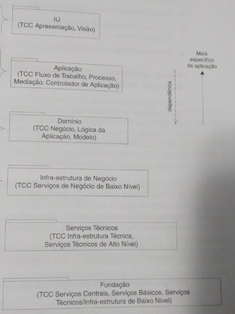
\includegraphics[keepaspectratio=true,scale=0.5]{figuras/arqcamadas.jpg}
	\caption{exemplo de arquitetura em camadas, Larman (2005, pg 225)}
\end{figure}

Já uma arquitetura orientada a componentes separam as funcionalidades em pacotes e o disponibilizam para uso por qualquer outro componente. Um componente, módulo ou pacote é um sub-conjunto de classes que realizam uma tarefa específica e centralizam nela toda a responsabilidade por lidar com isso. O componente em geral trabalha de forma caixa-preta, não fornecendo acesso a detalhes de implementação da solução. Szyperski (2002) define um componente como "uma entidade de composição com interfaces especificadas contratualmente e somente explícita no contexto da dependência. Um componente de software pode ser desenvolvido pelo próprio usuário como parte do sistema ou um módulo de terceitos com o qual se comunica". Szyperski (2002) também defende que cada módulo deve ser o mais independente possível e nem possuir um estado observável externamente.

Goodlife (2007) trás também outros dois padrões de arquitetura: cliente e servidor e \textit{pipe-and-filter}. A arquitetura cliente-servidor é muito usada em redes e sistemas distribuídos, aonde um programa requisita dados e/ou serviços de outro. O servidor provê uma série de serviços bem definidos e uma interface conhecida para receber as requisições de serviço. O cliente consome esses serviços e deve conhecer a interface do servidor para saber como pedir um dado ou serviço. A arquitetura \textit{pipe-and-filter} define todo componente como um filtro, que recebe um dado, trata-o e o repassa para outro filtro. Todo componente funciona com um dado de entrada e liberando um de saída. As interações entre os filtros são chamadas de \textit{pipes}. Um exemplo é o terminal do Linux, aonde pode dar vários comandos na mesma linha separados pela barra vertical (\textit{pipe}) e o resultado de um serve de entrada para o seguinte.

Independente da abordagem, as boas práticas de projeto (GRASP) os padrões de projeto de Gamma (1995) são seguidos para garantir a acoplamento, coesão, reusabilidade e clareza do código. O uso de polimorfismo e interfaces é incentivado e abstração vista como ponto chave do projeto da arquitetura. Szyperski (2002) diz que a abstração é talvez a mais poderosa ferramenta para um engenheiro de software. A abstração encapsula o problema em uma visão simplificada e assim deve se manter. "Encapsulamento diz que você não só está permitido a ter uma visão simplificada, diz que você não está permitido a ver mais detalhes que os fornecidos. O que você vê é tudo o que você tem" (McConnel, 2004, pg 91).

Também é comum à construção de qualquer arquitetura a divisão das tarefas em dois grupos: módulos (ou camadas) e suas interações. Definir como as funcionalidades estarão estruturadas e separá-las em módulos é só metade do trabalho, precisando haver um esforço em como elas se comunicarão e que essas comunicações sejam a mais simples possíveis. Szyperski (2002) também diz que o maior esforço dos arquitetos de software é em diminuir a complexidade das interações dos objetos. Quanto maior a interação, mais o acoplamento cresce e é algo a ser evitado ao máximo.

\subsection{Padrões de projeto}

Padrões de projeto são descrições de objetos e classes comunicantes que precisam ser personalizadas para resolver um problema geral de projeto num contexto particular (Gamma, 1995, pg 20). Esses padrões são soluções eficientes para problemas corriqueiros no desenvolvimento de software. Gamma (1995) catalogou estes padrões e descreveu cada um, juntamente com seu problema, em seu livro, fornecendo uma biblioteca de padrões bem aceitos e difundidos na comunidade.

Todo padrão possui o nome, o problema, sua solução e as consequências de sua implementação. Eles são divididos em finalidades: padrões de criação, estruturais e comportamentais.

Em um projeto de \textit{framework} certos padrões se destacam. O padrão \textit{Template Method} é destacado por Larman (2005) e Fayad (1999) por fornecer pronto a estrutura padrão para esse tipo de operação com as características constantes já implementadas e permitir a implementação daquilo que é diferente no contexto do sistema. O padrão Fachada também é comentado por Larman (2005) por fornecer uma interface única e simples para uma tarefa que usa várias classes e objetos. O princípio de Hollywood ou princípio da Inversão de Controle (implementado pelo padrão Injeção de Dependência) também é mencionado por Larman (2005) por diminuir o acoplamento entre as camadas e forçar a comunicação por interfaces, que dá um comportamento mais geral e também é outro princípio de boa programação.

Outros padrões comentados por Larman (2005) e Szyperski (2002) por serem muito utilizados em \textit{frameworks} são o \textit{Observer}, \textit{Command}, \textit{Composite}, \textit{Strategy} e \textit{Decorator}. Gamma (1995) descreve detalhadamente todos estes padrões.

\subsection{Caixa-preta e Caixa-branca}

Szyperski (2002) descreve \textit{frameworks} e componentes como podendo ser caixa-preta, caixa-branca ou caixa-cinza. Um \textit{framework} caixa-preta só revela suas interfaces e como usa-la. Neste tipo de abordagem não há nenhum tipo de informação sobre seu comportamento ou subclasses. Essa abordagem é raramente usada para \textit{frameworks} e mal aconselhada pelo autor, se encaixando melhor para projeto de componentes. Szyperski (2002) e Fayad (1999) dizem que, ainda assim, o sismtema caixa-preta não é todo fechado a extensão. Novos comportamentos podem ser adicionados através de \textit{plugins} que extendem das interfaces e unidos via composição. Porém Fayad (1999) também comenta que este tipo de abordagem é mais difícil de desenvolver.

Já a abordagem caixa-branca revela sua estrutura, permite extensão de suas classes e personalização de seu comportamento. Ela é muito mais usada para \textit{frameworks} e aconselhada por Szyperski (2002). Já Fayad (1999) diz que, apesar de ser largamente utilizado, a estrutura caixa-branca exige que o programador conheça profundamente a estrutra interna do \textit{framework} e que o uso de herança é muito mais comum em caixa-branca, enquanto no caixa-preta usa-se mais composição e delegação. Em comparação com o modelo caixa-preta, este é mais fácil de se desenvolver, porém mais difícil de extender.

O padrão caixa-cinza revela alguns detalhes de seu funcionamento e permite extensão e colaboração com alguns de seus pacotes, porém mantém algumas partes totalmente fechadas em seus componentes. \textit{Frameworks} caixa-cinza tem flexibilidade suficiente e extensibilidade, e ainda tem a habilidade de esconder informações desnecessárias do desenvolvedor da aplicação (Fayad, 1999, pg 10). 

\subsection{Hot-spot e Frozen-spot}

\textit{Frameworks} são adaptados para personalização e extensão das estruturas que provê. As partes do \textit{framework} abertas para extensão e personlaização são chamadas de \textit{hot-spot} (Fayad, 1999, pg 33). \textit{Hot-spots} expressam aspectos variantes do domínio e devem ser levantadas na fase de análise da construção do \textit{framework}. \textit{Hot-spots} são uma parte muito importante do \textit{framework}, pois são neles que o usuário tem a chance de construir algo. \textit{Hot-spots} deixam ganchos para que o usuário herde de interfaces e defina seus próprios comportamentos.

\textit{Frozen-spot}, por sua vez, são blocos fechados do \textit{framework}. São componentes que não permitem extensão e são apenas utilizados pelo restante. Enquanto um \textit{hot-spot} está semi-pronto o \textit{frozen-spot} já está pronto para uso e não pode ser alterado.

Determinar quais são os \textit{hot-spots} é uma das principais tarefas do desenvolvedor de \textit{frameworks}. Cada \textit{hot-spot} deve possuir uma interface da qual herdará. Essa interface serve para padronizar a comunicação e definir qual deve ser o comportamento daquele módulo. O \textit{framework} pode ou não vir com alguma implementação padrão e básica da interface.

Cada \textit{hot-spot} deve ser bem especificado pelo desenvolvedor do \textit{framework} para que o usuário saiba como construir suas customizações. Fayad (1999) defende que uma profunda análise do domínio e dos \textit{hot-spots} devem ser realizados, realzando e documentando uma análise alto nível dos \textit{hots spots}, uma especificação mais aprofundada dessas tarefas, o desenho alto nível de seus subsistemas e por fim codificar este desenho em uma classe abstrata e generalizações (se houver). Em um \textit{framework} caixa-preta deve haver uma série de implementações da interface já prontas para o usuário escolher qual utilizar enquanto no \textit{framework} caixa-branca o usuário deve desenvolver sua própria classe. Isso pode ser trabalhoso se a documentação da interface estver mal feita ou incompleta. A imagem abaixo ilustra a diferença entre as duas abordagens quanto aos ganchos \textit{hot-spot}.

\begin{figure}[h]
	\centering
	\label{fig12}
		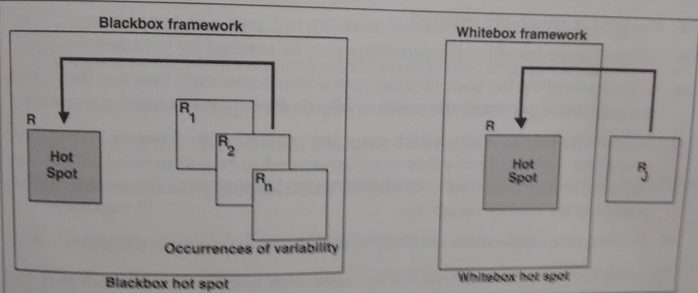
\includegraphics[keepaspectratio=true,scale=0.3]{figuras/hotspotbox.jpg}
	\caption{\textit{hot-spot} em um \textit{framework} caixa-preta e caixa-branca. Fayad (1999, pg 357)}
\end{figure}

Um subsistema \textit{hot-spot} pode conter apenas a classe base e suas extensões (subsistema baseado em herança) ou pode ter ainda classes adicionais e relacionamentos internos (subsistema baseado em composição). A primeira costuma-se usar o Padrão Fábrica ou \textit{Template} para comunicação externa, enquanto o subsistema por composição, que é mais complexo, exige um padrão mais complexo também, como o \textit{Strategy}.

Fayad (1999) classifica os subsistemas \textit{hot-spot} em três categorias de acordo com o número e estrutura das subclasses que possui. Ela pode ser não-recursiva se o serviço é realizado por apenas uma subclasse (o caso normal), recursão estruturada em cadeia (\textit{chain-structured recursive}) caso o serviço possa ser realizado por várias subclasses estrutradas em cadeia ou recursiva estrutrada em árvore (\textit{tree-structured recursive}) caso o serviço possa ser realizado por uma árvore de várias subclasses. Essa estrutura não é observável de fora do subsistema, que ao receber uma mensagem chama recursivamente os objetos (no caso de ser recursivo) através de um método \textit{Template} até percorrer toda a lista de objetos filhos ou chegar na folha da árvore. O tipo de um subsistema \textit{hot-spot} é definido pelo padrão de projeto implementado. Cada padrão provê variabilidade e flexibilidade de um modo diferente, causando as diferenças entre as três categorias citadas acima. Os não-recursivos são implementações de \textit{Interface Inheritance, Abstract Factory, Builder, Método Fábrica, Protótipo, Strategy, Template, Visitor, Adapter, Bridge, Proxy, Command, Iterator, Mediator, Observer} e \textit{State}. O recursivo estruturado em cadeia implementado com \textit{Chain of Responsability} e \textit{Decorator} e o recursivo estruturado em árvore implementado com \textit{Composite} e \textit{Interpreter}.

\begin{figure}[h]
	\centering
	\label{fig13}
		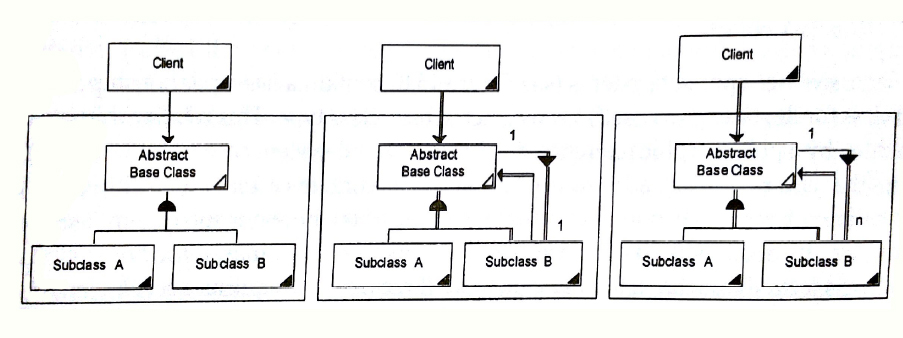
\includegraphics[keepaspectratio=true,scale=0.4]{figuras/subsistemaHotspot.jpg}
	\caption{Estruturas dos subsistemas \textit{hot-spot}. Fayad (1999, pg 363 e 364)}
\end{figure}

Em resumo, um \textit{framework} caixa-branca costuma ser baseado em herança ou interfaces, enquanto um caixa-preta é baseado em composição. Apesar das diferenças entre as duas, ambas possuem em sua estrutura interna superclasses e subclasses utilizadas para solucionar um problema, mudando como o usuário do \textit{framework} pode se comunicar com essas classes (herdando ou compondo-as em suas próprias classes). Em ambos os casos o padrão \textit{Template Method} é fortemente usado. O uso deste padrão fornece ganchos para inserir seus próprios comportamentos, sendo por isso este padrão comumente ligado a \textit{hot-spots}. Locais aonde o comportamento varia de aplicação para aplicação e o \textit{framework} se abre para que o usuário defina o comportamento é a definição de um \textit{hot-spot}, e também exatamente o que o padrão permite realizar. Quando um módulo possui uma série de objetos semelhantes ou com funções semelhantes o \textit{framework} pode criar uma estrutura recursiva em cadeia ou árvore (ao invés da referência direta) para guardá-los e manter as chamadas a eles.

\subsection{Processo de desenvolvimento orientado a hot-spots}

Um bom \textit{framework} nunca é feito de uma vez. A modelagem do domínio, análise dos pontos de variação e seu projeto são atividades iterativas, sendo sempre incrementadas e aperfeiçoadas. Assim, a modelagem de um \textit{framework} é uma tarefa iterativa e incremental, sendo constantemente alterada, melhorada e acrescentada novos \textit{hot-spots}. Os já existentes são avaliados se foram corretamente projetados e se fornecem abertura suficiente para personalização pelo usuário e mantêm o baixo acoplamento e a alta coesão. Todo esse processo gira em torno dos \textit{hot-spots}, permanecendo até que todo o modelo de domínio tenha sido esmiuçado e os \textit{hot-spots} levantados tenham sido analisados, projetados e implementados. A imagem a seguir esboça o fluxo de trabalho do processo orientado aos \textit{hot-spots}.

\begin{figure}[h]
	\centering
	\label{fig14}
		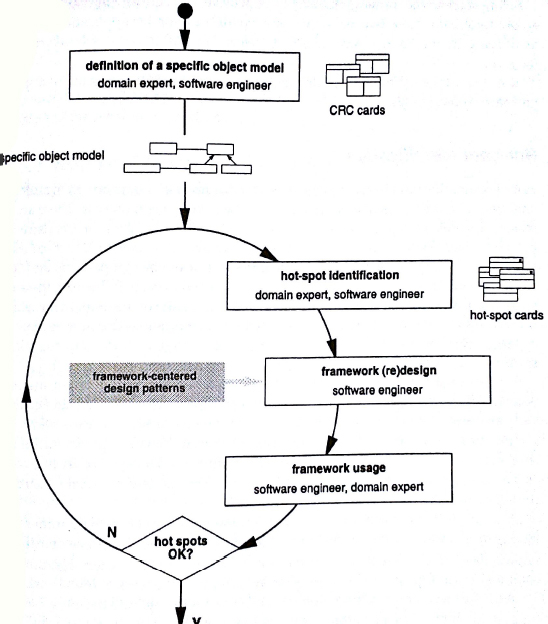
\includegraphics[keepaspectratio=true,scale=0.4]{figuras/hotspotdd.jpg}
	\caption{Processo de desenvolvimento orientado a \textit{hot-spot}. Fayad (1999, pg 385)}
\end{figure}

A definição de um específico modelo de objeto é a defiição exta do escopo do \textit{framework}, a construção de seu modelo de domínio e levantamento de requisitos. A cada porção do domínio levantada é identificado \textit{hot-spots}. Essa atividade é realizada tanto com o engenheiro de software quanto com um especialista no domínio tratado, que conhece das variancias do assunto. A comunicação do engenheiro com o expecialista pode ser complicada pelo specialista conhecer da área, porém desconhecer sobre classes, objetos, herança e hot-spots. Para facilitar a comunicação entre os dois e a identificação de novos \textit{hot-spots} Fayad (1999) sugere a utilização de \textit{hot-spot cards}.

O projeto e reprojeto do \textit{framework} ocorre após que os \textit{hot-spots} tiverem sido identificados e documentados. Essa atividade trata de projetar a abstração do \textit{hot-spot}, permitindo a extensibilidade no módulo e manter acoplamento baixo e a coesão alta. Padrões de projeto são utilizados para alcançar este fim. É nesta atividade que é analisado se o \textit{hot-spot} será não-recursivo ou recursivo a partir das decisões de projeto. A constante reavaliação dos \textit{hot-spots} e possívei reprojetos podem ocorrer em futuras iterações se forem identificados problemas na modelagem atual.

A última atividade da iteração é por fim implementar as decisões arquiteturais e de projeto da atividade anterior e seu uso afim de detectar falhas no mesmo. Vale lembrar que o projeto e a implementação seguem os \textit{hot-spot cards} como guia, que lhes dá uma forte tendência de como realizar aquele \textit{hot-spot}.

Um \textit{hot-spot card} contém informações sobre a semântica e o desejado grau de flexibilidade, mas não sobre qual classe o \textit{hot-spot} pertence (Fayad, 199, pg 388). Passar da análise para algo com valor arquitetural se torna relativamente simples com essa abordagem, pois o autor fornece uma relação de como implementar de acordo com o grau de flexibilidade. Porém essa integração depende de uma boa granularidade da função \textit{hot-spot}. Uma função \textit{hot-spot} com a granularidade correta implica que um método de gancho ou um grupo deles tem que ser adicionado. O local onde inserir o método gancho depende do grau de flexibilidade.

\begin{figure}[h]
	\centering
	\label{fig15}
		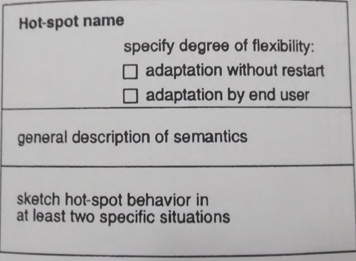
\includegraphics[keepaspectratio=true,scale=0.4]{figuras/hotspotcard.jpg}
	\caption{\textit{hot-spot card}. Fayad (1999, pg 387)}
\end{figure}

Caso ambas as opções de grau de flexibilidade estejam desmarcadas um método gancho deve ser adicionado (caso normal do método \textit{Template}). Caso a primeira opção seja marcada (sem reinício) esse método gancho deve ser implementado em uma classe gancho separada (gerando indireção para uma melhor abstração). Caso a segunda opção seja marcada (adaptação pelo usuário final) deve-se realizar uma forma de configuração do uso do método ou classe gancho. Com os dois selecionados, ambos, configuração e indireção, devem ser feitos.

\subsection{Abordagem de projetos}

Szyperski (2002) mostra outra maneira de projetar um \textit{framework}, mais simples e com menos foco em \textit{hot-spots}. Segundo ele o projeto de \textit{frameworks} pode ter duas abordagens: \textit{bottom up} (orientado a padrões) ou \textit{top down} (orientado a alvos).

A abordagem \textit{bottom up} funciona bem aonde o domínio já é bem entendido e conhecido. Por já se conhecer os problemas e ter uma boa visão de como será o final os componentes vão sendo desenvolvidos e os problemas atacados sem demora. Padrões são usados para o desenvolvimento dos componentes e para suas interações, o que dá seu outro nome (orientado a padrões). Os módulos são desenvolvidos até ter resolvido todos os problemas e conectado-os corretamente. Isso pode levar a uma codificação exagerada, indo além do necessário e fornecendo um monte de soluções fragmentadas e sem foco definido.

A abordagem \textit{top down} é preferível aonde o domínio ainda não foi suficientemente explorado, mas os problemas a serem resolvidos estão bem definidos. Em vez de focar na solução e sua implementação como o anterior, este foca nos problemas e vai construindo a solução a partir deles, por isso o nome orientação a alvos. Neste contexto, um alvo é definido como um conjunto de entidades e interações encontradas em \textit{frameworks} já implementados que demonstram um bom resultado.

\section{Trabalhos relacionados}

A ideia de criar um \textit{framework} para abstrair o código e permitir o reuso entre kits diferentes não é algo novo. A comunidade de robótica já sentiu a necessidade de uma forma de adaptar seus programas e criou sistemas semelhantes ao sugerido neste trabalho.

A seguir será apresentado dois \textit{frameworks} para desenvolvimento de robôs: O Carmen e o ROS, que implementam diversos módulos do funcionamento da robótica móvel, entre elas a navegação e definição de trajetória. É apresentado também uma tese de PhD que apresenta um \textit{framework} para desenvolvimento e avaliação de algoritmos de definição de trajetória.

O diferencial deste trabalho aos demais é funcionar em linguagem Java, dando suporte para o desenvolvimento em uma nova linguagem e seguindo as boas práticas de programação da engenharia de software, torando o código-fonte mais fácil de compreender e mais manutenível. Além disto pouquíssimos \textit{frameworks} funcionam no kit educacional da LEGO.

\subsection{Carmen}

O Carmen (Carnegie Mellon Robot Navigation Toolkit) é um \textit{framework} \textit{open-source} para controle de robôs móveis. Ele é focado em toda parte de navegação, dando uma coleção volumosa para o desenvolvimento de novos programas. Ele é escrito predominantemente e C e possui uma arquitetura modular que trocam informações através de IPC (\textit{inter proccess comunication}). Suas principais funcionalidades incluem: sensoriamento, \textit{logging}, desvio de obstáculos, localização, definição de trajetória e mapeamento (http://carmen.sourceforge.net/intro.html). 

O Carmen funciona em uma série de robôs diferentes, permitindo portabilidade entre os hardwares com qual trabalha. Entre eles estão o IRobot, ActivMedia Pioneer, OrcBoard e SegWay.

O Carmen monta o mapa como uma malha de ocupação, formando uma matriz com os espaços ocupados e livres. Para definição de trajetória o \textit{frmaework} usa um algorítmo potencial chamado Konoliges Linear Programming Navigation \textit{gradient method} ou LPN (Thomsen, 2010).

\subsection{ROS}

O ROS (Robot Operating System) é um \textit{framework} \textit{open-source} que trabalha como um sistema operacional, abstraindo o hardware para o usuário e fornecendo um controle de dispositivos de baixo nível. O \textit{framework} fornece ainda fácil troca de mensagens entre processos, gerenciamento de pacotes e funcionamento em nós, permitindo a execução de código em vários computadores (http://wiki.ros.org/ROS). O \textit{framework} também possui uma gama de ferramentas e bibliotecas para simulação e teste do código. O código está disponível em C++ e Python para desenvolvimento em qualquer uma da sduas linguagens. Dentre os hardwares em que ele funciona estão o Aldebaran Nao, Robotnik Guardian, Neobotix, AscTec Quadrotor, entre outros.

\subsection{Tese de Morten Strandberg}

Morten Strandberg (2004) realiza em sua tese de phd um framework que facilita na criação e avaliação de planejadores de caminho. Seu trabalho não se restringe apenas à robótica móvel, mas qualquer aplicação que use de planejadores de caminho, embora seu foco seja na robótica industrial. Ele considera o ambiente onde o robô estará como dinâmico, ou seja, os obstáculos podem se mover.

Strandberg (2004) divide os conceitos em quatro grupos: representação geométrica dos obstáculos, a detecção de colisão, o planejamento da trajetória e os modelos de movimento do robô. Com isso é perceptível que o trabalho vai além de puramente definir a trajetória, pois lida com o sensoriamento constante e a atuação dos motores para movimentação do robô.

O framework foi construído a partir das técnicas de orientação a objetos e de padrões de projeto, visando a fácil estenção, usabilidade, portabilidade e o baixo acoplamento. Para isso o autor definiu um conjunto de componentes, cada um com uma responsabilidade diferente. Cada componente possui uma hierarquia de classes de baixo acoplamento que realizam as tarefas, baseadas em uma interface comum a todo o componente. Essa interface facilita uma comparação justa entre diferentes implementações de definição de trajetória.

As métricas são feitas a partir de cálculos sobre a posição dos objetos e do ambiente. Quase todas as métricas são feitas a partir de uma equação como a métrica Manhattan ou a de corpo rígido. As métricas e suas variações também formam um módulo do sistema, com sua própria hierarquia de classes e uma classe abstrata mãe que serve de interface para o resto do sistema.